\documentclass[a4paper, 11pt]{article}
\usepackage{comment}
\usepackage{lipsum} 
\usepackage{fullpage} %cambiar margen
\usepackage[a4paper, total={7in, 10in}]{geometry}

\usepackage{amssymb,amsthm} 
\usepackage{amsmath}
\newtheorem{theorem}{Theorem}
\newtheorem{corollary}{Corollary}
\usepackage{graphicx}
\usepackage{tikz}
\usetikzlibrary{arrows}
\usepackage{verbatim}
%\usepackage[numbered]{mcode}
\usepackage{float}
\usepackage{tikz}
\usetikzlibrary{shapes,arrows}
\usetikzlibrary{arrows,calc,positioning}
\usepackage{mathpazo} %tipo de letra 
\usepackage[utf8]{inputenc} %codificación
\usepackage[T1]{fontenc} %digitación de tildes y ñ
\usepackage[spanish]{babel} %paquete de soporte español

\tikzset{
	block/.style = {draw, rectangle,
		minimum height=1cm,
		minimum width=1.5cm},
	input/.style = {coordinate,node distance=1cm},
	output/.style = {coordinate,node distance=4cm},
	arrow/.style={draw, -latex,node distance=2cm},
	pinstyle/.style = {pin edge={latex-, black,node distance=2cm}},
	sum/.style = {draw, circle, node distance=1cm},
}
\usepackage{xcolor}
\usepackage{mdframed}
\usepackage[shortlabels]{enumitem}
\usepackage{indentfirst}
\usepackage{hyperref}

\usepackage{listings}
\lstset{literate=
  {á}{{\'a}}1
  {é}{{\'e}}1
  {í}{{\'i}}1
  {ó}{{\'o}}1
  {ú}{{\'u}}1
  {Á}{{\'A}}1
  {É}{{\'E}}1
  {Í}{{\'I}}1
  {Ó}{{\'O}}1
  {Ú}{{\'U}}1
  {ñ}{{\~n}}1
  {ü}{{\"u}}1
  {Ü}{{\"U}}1
}

\lstdefinestyle{customc}{
  belowcaptionskip=1\baselineskip,
  breaklines=true,
  frame=L,
  xleftmargin=\parindent,
  language=Python,
  showstringspaces=false,
  basicstyle=\footnotesize\ttfamily,
  keywordstyle=\bfseries\color{green!40!black},
  commentstyle=\itshape\color{purple!40!black},
  identifierstyle=\color{blue},
  stringstyle=\color{orange},
}

\lstdefinestyle{customasm}{
  belowcaptionskip=1\baselineskip,
  frame=L,
  xleftmargin=\parindent,
  language=[x86masm]Assembler,
  basicstyle=\footnotesize\ttfamily,
  commentstyle=\itshape\color{purple!40!black},
}

\lstset{escapechar=@,style=customc}



\renewcommand{\thesubsection}{\thesection.\alph{subsection}}

\newenvironment{problem}[2][Ejercicio]
{ \begin{mdframed}[backgroundcolor= red!50] \textbf{#1 #2} \\}
	{  \end{mdframed}}

% Define solution environment
\newenvironment{solution}
{\textcolor{blue}{\textbf{\textit{Solución:\\\noindent}}}}


\renewcommand{\qed}{\quad\qedsymbol}

% \\	
\begin{document}
	\noindent
	%%%%%%%%%%%%%%%%%%%%%%%%%%%%%%%%%%%%
	
	\begin{minipage}[b][1.2cm][t]{0.8\textwidth}
		\large\textbf{César Isaí García Cornejo} \hfill \textbf{Tarea 1}  \\
		cesar.cornejo@cimat.mx \hfill \\
		\normalsize Series de Tiempo \hfill Semestre 3\\
	\end{minipage}
	
	\hspace{14.4cm}
	\begin{minipage}[b][0.03cm][t]{0.12\linewidth}
		
		\vspace{-2.2cm}
		%%%La Ruta depeendera de donde este alojado el main y la imagen
		
\includegraphics[scale=0.3]{Figures/EscudoCimat.png}
	\end{minipage}
	
	\noindent\rule{7in}{2.8pt}
	
	%%%%%%%%%%%%%%%%%%%%%
	%%%%%%%%%%%%%%%%%%%%%%%%%%%%%%%%%%%%%%%%%%%%%%%%%%%%%%%%%%%%%%%%%%%%%%%%%%%%%%%%%%%%%%%%%%%%%%%%%%%%%%%%%%%%%%%%%%%
	% Problem 1
	%%%%%%%%%%%%%%%%%%%%%%%%%%%%%%%%%%%%%%%%%%%%%%%%%%%%%%%%%%%%%%%%%%%%%%%%%%%%%%%%%%%%%%%%%%%%%%%%%%%%%%%%%%%%%%%%%%%%%%%%%%%%%%%%%%%%%%%%
	\setlength{\parskip}{\medskipamount}
	\setlength{\parindent}{0pt}
 %///////////////////////////////////////////////////
\begin{problem}{1}
    Considera la serie de tiempo $\{X_t\}$ contenida en la primera columna del archivo airline.csv. Dicho conjunto de datos consiste en los totales mensuales L en miles= de pasajeros internacionales de una aerolínea durante el período de enero de 1949 a diciembre de 1960 (ver Brockwell and Davis (1991)). Realiza lo siguiente: 
    \begin{enumerate}
        \item Gráfica la serie de tiempo (como función del tiempo). ?`Hay algunas tendencias obvias?
        \item ?` Es necesario transformar los datos? Si se require una transformación. ?`qué sugerirías?
        \item Calcula la mediana del número de pasajeros internacionales de cada año. Grafica simultáneamente boxplots del número de pasajeros en casa año para detectar cualquier otra tendencia. 
        \item Encuentra un estimado de la tendencia usando un filtro de medias móviles. Grafica la tendencia.
    \end{enumerate}
\end{problem}

\begin{solution}
  El enlace a los códigos del ejercicio 1 se encuentra
  \href{https://colab.research.google.com/drive/1INC0Hm5ToZ22szOR6O2550CCoFIQ1jXs?usp=sharing}{\color{blue}aquí}.

  Observamos de la Fig. \ref{Fig:1.1} que tenemos cierta tendencia a la alza según pasan los años. Además notamos estacional pues los picos y valles parecen equidistantes.


  \begin{figure}[H]
    \centering
    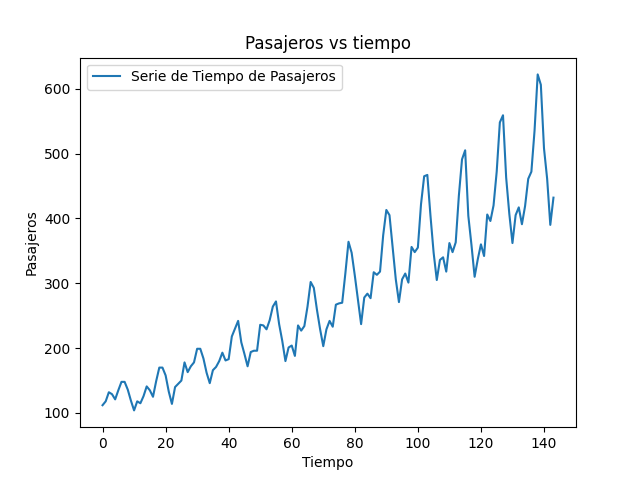
\includegraphics[width = 10 cm ]{Figures/S1.png}
    \caption{Serie de tiempo para los pasajeros de una aerolínea durante el periodo 1949 a 1960.}
    \label{Fig:1.1}
  \end{figure}

  Notemos tambien que la serie de tiempo incrementa en varianza conforme incrementa el tiempo. Se sugiere transformar dicha serie de tiempo tomando el logaritmo de los pasajeros, esta transformación hace al proceso homocedástico, como podemos ver el la Fig. \ref{Fig:1.2} y esta transformación no pierde su interpretabilidad.

  
  \begin{figure}[H]
    \centering
    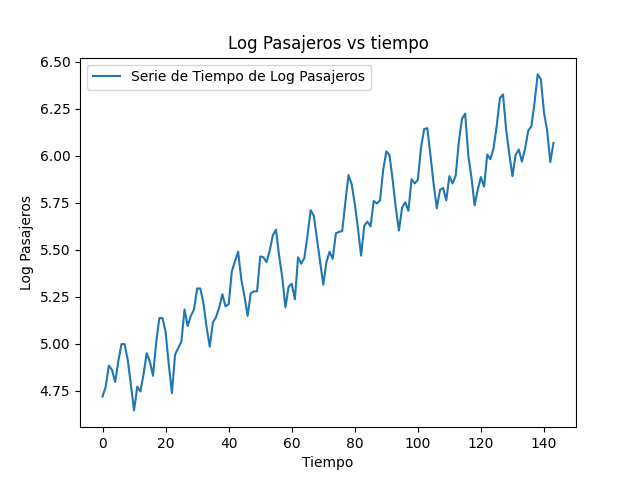
\includegraphics[width = 9 cm ]{Figures/S2.png}
    \caption{Serie de tiempo para el logaritmo de pasajeros de una aerolínea durante el periodo 1949 a 1960.}
    \label{Fig:1.2}
  \end{figure}


  Ahora del \textit{dataframe} seccionado usamos el metodo \textit{describe()} con lo que podemos obtener la media para cada año descrito en la tabla siguiente

  \begin{table}[H]
    \begin{center}
      \begin{tabular}{ll}
        \multicolumn{1}{c}{Año} & Mediana \\\hline
        1949                    & 125     \\
        1950                    & 137.5   \\
        1951                    & 169     \\
        1952                    & 192     \\
        1953                    & 232     \\
        1954                    & 231.5   \\
        1955                    & 272     \\
        1956                    & 315     \\
        1957                    & 351.5   \\
        1958                    & 360.5   \\
        1959                    & 406.5   \\
        1960                    & 461     \\ \hline
  \end{tabular}
  \caption{Mediana por año para la serie de los pasajeros}
  \label{tab:01}
    \end{center}
  \end{table}

  
  \begin{table}[H]
    \begin{center}
      \begin{tabular}{ll}
      \multicolumn{1}{c}{Año} & Mediana \\\hline
      1949                    & 4.83    \\
      1950                    & 4.92    \\
      1951                    & 5.13    \\
      1952                    & 5.26    \\
      1953                    & 5.44    \\
      1954                    & 5.44    \\
      1955                    & 5.60    \\
      1956                    & 5.75    \\
      1957                    & 5.86    \\
      1958                    & 5.88    \\
      1959                    & 6.01    \\
      1960                    & 6.13    \\ \hline
    \end{tabular}
    \caption{Mediana por año para la serie del logaritmo de los pasajeros}
    \label{tab:02}
  \end{center}
\end{table}

Notemos que de la Fig. \ref{Fig:1.3} tenemos que tienden a tener colas más grandes. Luego la varianza incrementa tal como se afirmó previamente. Además, de la Fig. \ref{Fig:1.4} notemos que está no varia en covarianza pues los boxplots parecen tener la misma longitud.

\begin{figure}[H]
  \centering
  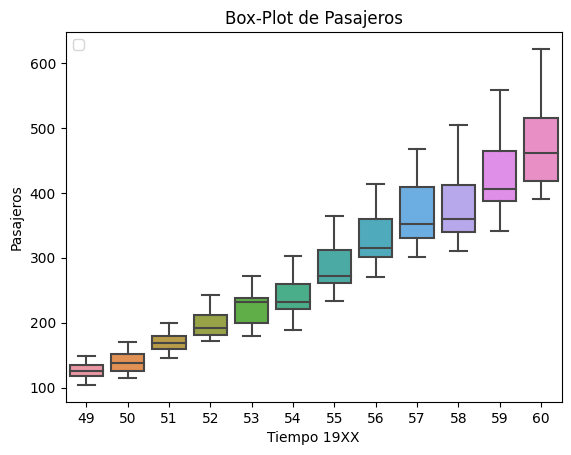
\includegraphics[width = 10 cm ]{Figures/Boxplot1.png}
  \caption{Box-plot de los pasajeros durante los 12 meses a cada año del periodo para los pasajeros.}
  \label{Fig:1.3}
\end{figure}


\begin{figure}[H]
  \centering
    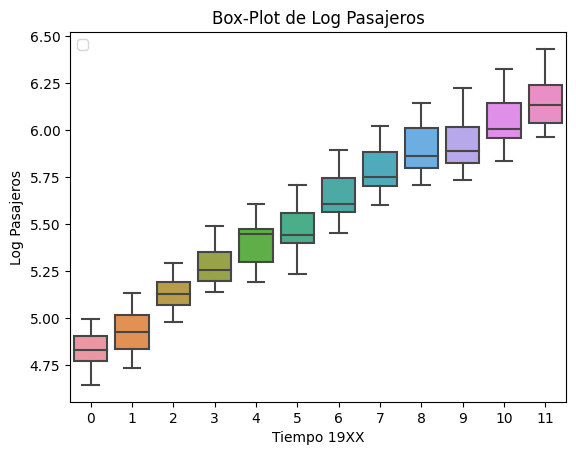
\includegraphics[width = 10 cm ]{Figures/Boxplot2.png}
    \caption{Box-plot de el logaritmo de pasajeros durante los 12 meses a cada año del periodo para los pasajeros.}
    \label{Fig:1.4}
\end{figure}


Por último, encontramos la estimación de la tendencia del modelo por medio de \textbf{medias moviles}. Es decir, consideramos el estimador de $T$ en $ X_t = T_t + e_T$ como
\begin{align*}
  \hat{T }_t = \frac{1}{2q+1}\sum_{j=-q }^{q }X_{t+j}
\end{align*}
que es el filtro de media movil uniforme (mismos pesos). La implementación del código en python es como sigue.
\begin{lstlisting}

  def MediaMovil(datos,q):
  
  n = len(datos)
  T_hat = np.zeros(n-2*q)
  for i in range(n-2*q):   #Calcular el promedio de los 2q+1 valores consecutivos en la serie temporal.
      aux = 0
      for j in range(2*q + 1):
          aux += datos[j + i ]

      T_hat[i] = aux/(2*q+1)
  
  x = np.linspace(q,n-2*q-1,n-2*q)  #Linspace para gráficar
  return x, T_hat
\end{lstlisting}

Ingresando en la función constuida el vector tipo arreglo numpy y el numero de puntos $q =8$ tenemos los siguientes filtros para el caso de la serie temporal de los pasajero y la serie temporal transformada del logaritmo de los pasajeros en la Fig. \ref{Fig:1.5}  y la Fig. \ref{Fig:1.6} 


\begin{figure}[H]
  \centering
    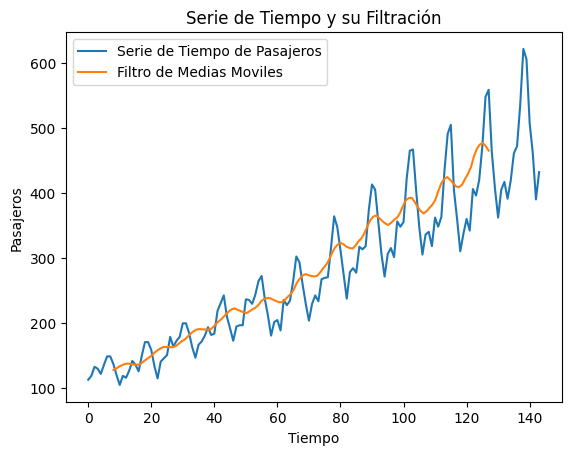
\includegraphics[width = 9 cm ]{Figures/MediaMovil.png}
    \caption{Serie de tiempo de los pasajeros y su filtración para la tendencia por medias moviles con $q = 8$.}
    \label{Fig:1.5}
\end{figure}

\begin{figure}[H]
  \centering
    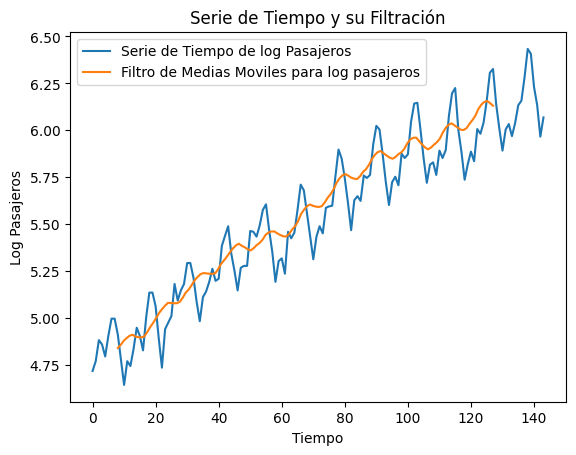
\includegraphics[width = 9 cm ]{Figures/LogMediaMovil.png}
    \caption{Serie de tiempo de el logaritmo de los pasajeros y su filtración para la tendencia por medias moviles con $q = 8$.}
    \label{Fig:1.6}
\end{figure}
\end{solution}



%///////////////////////////Ejercicio ////////////////////////
\begin{problem}{2}
    Suponga que $\{e_t, t = 0,\pm 1, \pm 2, ...  \}$ es una sucesión de v.a.i.i.d. (0,$\sigma^2$). Calcula $\mathbb{E}[X_t]$ y $Cov(X_t,X_{t+h})$ para toda $t$ y para toda $h$ para los siguientes procesos estocásticos $\{X_t\}$.
    \begin{enumerate}
        \item $X_t = e_t e_{t-1}$, $t= 0,\pm 1, \pm 2,...$
        \item 
        $$
        X_t = \left\{\begin{matrix}
        \!\!\!\!\!\!\!\!\!  0 \:\:\:\:\:\:\:\:\:\:\:\:\:\:\:\:\:\:\:   t =0\\ 
        X_{t-1} + e_t \:\:\:\:\:\:\:\:\:\:  t =1,2,3,...
        \end{matrix}\right.
        $$
        \item $X_t = a_1 + e_1a_2^t+e_2$ para $a_1 \in \mathbb{R}$. $0 < a_2 < 1$. $t = 0,1,2,...$
        \item 
        $$
        X_t = \left\{\begin{matrix}
        \!\!\!\!\!\!\!\!\!  e_0 \:\:\:\:\:\:\:\:\:\:\:\:\:\:\:\:\:\:\:   t =0\\ 
        X_{t-1} + e_t \:\:\:\:\:\:\:\:\:\:  t =1,2,3,...
        \end{matrix}\right.
        $$
        \item Sea $X_0 \sim N(0,\sigma^2)$ una v.a. independiente de $\{e_t\}$. Define
        $$
        X_t = \left\{\begin{matrix}
        \!\!\!\!\!\!\!\!\!  X_0 \:\:\:\:\:\:\:\:\:\:\:\:\:\:\:\:\:\:\:   t =0\\ 
        \rho X_{t-1} + e_t \:\:\:\:\:\:\:\:\:\:  t =1,2,3,...
        \end{matrix}\right.
        $$
        \item $X_t = 0.5  e_1 + 1.5 e_2t$. para $0 \leq t \leq 1$. 
        \item $X_t = 0.4 +(-1)^t e_t$. para $t= 0,\pm1, \pm2,...$
        \item $X_t = e_2 cos t +e_3 sin t + e_t$. para $t= 4,5,6,....$
    \end{enumerate}
\end{problem}

\begin{solution}
\begin{enumerate}
  \item Para la esperanza de este proceso estocástico usamos la independencia del ruido blanco. Así 
  \begin{align*}
    \mathbb{E}[X_t] &= \mathbb{E}[e_t e_{t-1}],\\
    &= \mathbb{E}[e_t]\mathbb{E}[e_{t-1}],  \\  &= 0
  \end{align*}
  Luego, para la covarianza es necesario observar por casos. Tenemos que
  \begin{align*}
    Cov(X_t,X_{t+h}) 
  \end{align*}
  para $h= 0$ 
  \begin{align*}
    Cov(X_t,X_{t}) & = \mathbb{V}ar[X_t],\\
    &= \mathbb{E}[X_t^2] - \mathbb{E}^2[X_t], \\
    &= \mathbb{E}(e_t^{2} e_{t-1}^2],\\         %
    &= \mathbb{E}[e_t^2]\mathbb{E}[e_{t-1}^2],\\
    &= \left(\mathbb{E}[e_t^2] - \mathbb{E}^2[e_t]\right) \left(\mathbb{E}[e_{t-1}^2] - \mathbb{E}^2[e_{t-1}]\right),\\         %
    &= \sigma^4
  \end{align*}
  Posteriormente es necesario calcular para $h = 1$
  \begin{align*}
    Cov(X_t,X_{t+1}) &= \mathbb{E}[(e_te_{t-1})(e_{t+1}e_{t})],\\ &= \mathbb{E}[e^2_t]\mathbb{E}[e_{t-1}]\mathbb{E}[e_{t+1}] =0
  \end{align*}
  por independencia. De manera semejante para $h= -1$. Ahora, es necesario revizar para $h=\pm 2$, $h = \pm 3$ ,... y así sucesivamente .Sin embargo consideramos los casos restantes a la vez. Para $h \neq 0$
  \begin{align*}
    Cov(X_t,X_{t+h}) &= \mathbb{E}[e_te_{t-1}e_{t+h}e_{t-h+1}] ,\\
    &= \mathbb{E}[e_t]\mathbb{E}[e_{t-1}]\mathbb{E}[e_{t+h}]\mathbb{E}[e_{t-h+1}] = 0.
  \end{align*}

  Por tanto, concluimos que 
  \begin{align}
    Cov(X_t, X_{t+h}) = \sigma^4 \mathbb{1}_{h=0}
  \end{align}
  que es la covarianza para un ruido blanco.

  \item Construyamos una relación recursiva. Notemos que para $t = 0$ tenemos que $\mathbb{E}[X_0] = 0$. Para $t \geq 1$ se cumple que 
  \begin{align*}
    \mathbb{E}[X_t] = \mathbb{E}[X_{t-1}],
  \end{align*}
  por tanto, recursivamente 
  \begin{align*}
    \mathbb{E}[X_t] &= \mathbb{E}[X_{t-1}],\\
    &= \mathbb{E}[X_{t-2}],\\ 
    & \vdots\\
    &= \mathbb{E}[X_{0}] = 0.
  \end{align*}
  De manera semejante calculamos la covarianza. Para el caso $h=0$ y $t\geq 1$
  \begin{align*}
    \mathbb{V}ar[X_t] = \mathbb{V}ar[X_{t-1} + e_t] = \mathbb{V}ar[X_{t-1}] + \sigma^2
  \end{align*}
  Denotemos por $v_t = \mathbb{V}ar[X_t]$. Entonces,
  \begin{align*}
    v_t &= v_{t-1} +\sigma^2,\\
        &= v_{t-2} +2\sigma^2,\\
        &= v_{t-3} +3\sigma^2,\\
        \vdots\\
        &= v_0 + t\sigma^2,\\
        &= t\sigma^2.
  \end{align*}
  De la relación
  \begin{align}
    X_{t+h} = X_{t } + \sum_{j=1}^{h} e_{t+j}
    \label{2.01}
  \end{align}
  para $h > 0 $, que surge de la recursión
  \begin{align*}
    X_{t+h} &= X_{t+h-1} + e_{t+h}\\
    &= X_{t+h-2} + e_{t+h-1} + e_{t+h}\\
    & \vdots \\
    % &= X_{t+h-3} + e_{t+h-2} + e_{t+h-1} + e_{t+h}\\
    &= X_{t} + e_{t+1} + \cdots + e_{t+h-1} + e_{t+h},\\
    &= X_{t } + \sum_{j = 1}^{h } e_{t +j}
  \end{align*}
  Ahora consideramos $h\geq 1$.
  \begin{align*}
    Cov(X_t,X_{t+h}) &= Cov\left (X_t, X_t +\sum_{j=1}^{h} e_{t+j} \right ),\\
    & = Cov(X_t, X_t) + \sum_{j=1}^{h} Cov(X_t,e_{t+j}),\\
    & = \mathbb{V}ar[X_t ],\\
    & = t\sigma^2
  \end{align*}
  Ahora, para el caso $h <0 $. Sea $k = -h$ entonces se satisface
  \begin{align}
    X_{t } = X_{t-k } + \sum_{j = 1}^{k }e_{t-k+j }
    \label{2.02}
  \end{align}
  que se deriva del análisis de la recursión
  \begin{align*}
    X_t &= X_{t-1}  +e_t,\\ 
    &= X_{t-2} + e_{t-1} + e_t ,\\
    % &= X_{t-3} + e_{t-2} + e_{t-1} + e_t,\\
    &\vdots\\
    &= X_{t-k } + e_{t-k +1 } + \cdots + e_{t-1} + e_t,\\
    &= X_{t-k } + \sum_{j = 1 }^{k }e_{t-k +j}
  \end{align*}
  Entonces
  \begin{align*}
    Cov(X_t,X_{t-k}) &= Cov(X_{t-k }+\sum_{j = 1}^{k }e_{t-k+j},X_{t-k }),\\
    &= Cov(X_{t-k },X_{t-k }) +\sum_{j = 1}^{h} Cov(e_{t-k+j},X_{t-k }),\\
    &= (t-k )\sigma^2 
  \end{align*}
  para $t\geq k $. Para el caso $t<k$ por definición del proceso $Cov(X_{t},X_{t-k }) = 0$. 
  Por tanto, la covarianza es
  \begin{align*}
    Cov(X_t,X_{t+h }) &= \left\{\begin{matrix}
      t\sigma^2, & h\geq 0  \\ 
      (t+h) \sigma^2, & h<0, t+h\geq 0 
      \end{matrix}\right. \\&= \left (min\{t,t+h\}\right )^+\sigma^2
  \end{align*}
  donde el simbolo $(a)^+ = max\{a,0\} $.

  \item Para el siguiente caso tenemos 
  \begin{align*}
    \mathbb{E}[X_t] &= \mathbb{E}[a_1+ e_1 a_2^t +e_2],\\ &= a_1 + a_2^t\mathbb{E}[e_1] + \mathbb{E}[e_2],\\ &= a_1
  \end{align*}
  Luego,
  \begin{align*}
    Cov(X_t,X_{t+h }) &= Cov(a_1+ e_1 a_2^t +e_2,a_1+ e_1 a_2^{t+h} +e_2),\\
    &= Cov(e_1 a_2^t +e_2, e_1 a_2^{t+h} +e_2),\\
    &= Cov(e_1 a_2^t,e_1 a_2^{t+h}) + Cov(e_1 a_2^t,e_2) + Cov(e_2, e_2 a_2^{t+h}) + Cov(e_2,e_2),\\
    &= Cov(e_1 a_2^t,e_1 a_2^{t+h})+ Cov(e_2,e_2),\\
    &= \sigma ^2 (a_2^{2t+h} +1)
  \end{align*}
  para $t+h \geq 0$.

  \item Procedemos de manera semejante al inciso 2
  \begin{align*}
    \mathbb{E }[X_t ] &= \mathbb{E }[X_{t-1} ] + \mathbb{E}[e_t] , \\
    &= \mathbb{E }[X_{t-1}],\\
    &= \cdots\\
    &= \mathbb{E }[X_{0}] = 0
  \end{align*}
  Para la covarianza, de la relación (\ref{2.01}) se sigue para $h\geq 0$
  \begin{align*}
    Cov(X_t, X_{t+h} ) &= Cov\left (X_t, X_t + \sum_{j=1}^{h} e_{t+j}\right ),\\
    &= t\sigma^2
  \end{align*}
  De la relación (\ref{2.02}) tenemos que para $h<0$ con $k = -h$
  \begin{align*}
    Cov(X_t,X_{t-k }) = (t-k )\sigma^2
  \end{align*}
  para $k \leq t$. Obtenemos la misma relación de covarianza que en el inciso 2.

  \item 
  La variable inicial $X_0 \sim N(0,\lambda^2)$. Nuevamente, buscamos relaciones de recursión. Para la esperanza es simple pues
  \begin{align*}
    \mathbb{E}[X_t ] &= \mathbb{E }[\rho X_{t-1} + e_t ],\\
    &= \rho \mathbb{E }[X_{t-1}],\\
    &= \rho^2 \mathbb{E }[X_{t-2}],\\
    &\vdots\\
    &= \rho^t \mathbb{E }[X_0] = 0
  \end{align*}
  Para la covarianza, en el caso $h=0$ 
  \begin{align*}
    Cov(X_{t},X_t) &= \mathbb{V }ar[X_t ],\\ 
    &= \mathbb{V }ar[\rho X_{t-1} +e_t ],\\
    &= \rho^2 \mathbb{V }ar[X_{t-1}] + \sigma^2
  \end{align*}
  con la notación $v _t = \mathbb{V }ar[X_t ]$ tenemos la relación
  \begin{align}
    v_t &= \rho^2 v_{t-1} + \sigma^2,\nonumber\\
    &= \rho^2 (\rho^2 v_{t-2} + \sigma ^2 ) + \sigma^2,\nonumber\\
    &= \rho^4v_{t-2} + \rho ^2\sigma^2 + \sigma^2,\nonumber \\
    &= \rho^6 v_{t-3} + \rho^4\sigma^2 + \rho^2 \sigma^2+ \sigma^2,\nonumber\\
    &\vdots\nonumber\\
    &= \rho^{2t}v_{t-t} + \rho^{2(t-1)}\sigma^2 +\cdots + \rho^{2}\sigma^2 + \sigma^2,\nonumber\\
    &= \rho^{2t} \lambda^2 + \sigma^2 \frac{1-\rho^{2t}}{1-\rho^2}
  \end{align} 
  Ahora, análisemos para $h\geq 0$. Tenemos la relación
  \begin{align*}
    X_{t+h} = \rho^h X_t + \sum_{j=1}^{h }\rho ^{h-j} e_{t+j}
  \end{align*}
  que se obtiene de 
  \begin{align*}
    X_{t+h } &= \rho X_{t+h-1} + e_{t+h },\\
    &= \rho^2 X_{t+h-2} +\rho e_{t+h-1} + e_{t+h },\\
    & \vdots\\
    &= \rho ^h  X_t +\rho^{h-1}e_{t+1} + \rho^{h-2} e_{t+2} + \cdots + \rho e_{t+h-1} + e_{t+h }
  \end{align*}
  Entonces
  \begin{align*}
    Cov(X_t,X_{t+h }) &= Cov\left (X_t,\rho^h X_t + \sum_{j=1}^{h }\rho ^{h-j} e_{t+j} \right ),\\
    &= \rho ^h Cov(X_t,X_t) + \sum_{j=1}^{h }\rho ^{h-j} Cov(X_t,e_{t+j}),\\
    &= \rho ^h \left(\rho^{2t} \lambda^2 + \sigma^2 \frac{1-\rho^{2t}}{1-\rho^2}\right)
  \end{align*}
  Falta análizar el caso $h<0 $. Sea $k = -h$, tenemos la relación
  \begin{align*}
    X_t = \rho^k X_{t-k } + \sum_{j=1}^{k } e_{t-k+j}
  \end{align*}
  para $t\geq k$. Lo anterior se obtiene de
  \begin{align*}
    X_t &= \rho X_{t-1} + e_t,\\
        &= \rho\left(\rho X_{t-2} +e_{t-1}\right) + e_{t },\\
        &= \rho^2X_{t-2} + \rho e_{t-1} + e_t ,\\
        &\vdots\\
        &= \rho ^k X_{t-k } + \rho^{k-1} e_{t-k+1} + \cdots + \rho e_{t-1} +e_t 
  \end{align*}
  Se sigue
  \begin{align*}
    Cov(X_t,X_{t-k } ) &= Cov\left (\rho^k X_{t-k } + \sum_{j=1}^{k } e_{t-k+j} , X_{t-k }\right ),\\
    &= \rho^k Cov(X_{t-k },X_{t-k}) + \sum_{j=1}^{k } Cov(e_{t-k+j},X_{t-k }),\\
    &= \rho^k \mathbb{V }ar[X_{t-k }],\\
    &= \rho^k \left(\rho^{2(t-k) } \lambda^2 + \sigma^2 \frac{1-\rho^{2(t-k )}}{1-\rho^2}\right)
  \end{align*}
  Por tanto
  \begin{align*}
    Cov(X_t,X_{t+h}) = \left\{\begin{matrix}
      \rho ^h \left(\rho^{2t} \lambda^2 + \sigma^2 \frac{1-\rho^{2t}}{1-\rho^2}\right), &   h\geq 0 \\
      \rho^k \left(\rho^{2(t-k) } \lambda^2 + \sigma^2 \frac{1-\rho^{2(t-k )}}{1-\rho^2}\right), &   h<0
      \end{matrix}\right.
  \end{align*}
  con $k =-h$. Luego


  \begin{align*}
    Cov(X_t,X_{t+h}) = \left\{\begin{matrix}
      \rho^{2t+h} \lambda^2 + \sigma^2 \frac{\rho^h-\rho^{2t+h}}{1-\rho^2}, &   h\geq 0 \\
      \rho^{2t-k } \lambda^2 + \sigma^2 \frac{\rho^{k }-\rho^{2t-k }}{1-\rho^2}, &   h<0
      \end{matrix}\right.
  \end{align*}
  que se reduce a 
  \begin{align*}
    Cov(X_t, X_{t+h}) = \rho^{2t+h}\lambda^2 + \sigma^2 \frac{\rho^h - \rho^{2t+h}}{1-\rho^2} 
  \end{align*}
  para todo $h \in \mathbb{R}$

  


  \item Calculando directamente de $X_t = 0.5e_1 + 1.5e_2t$
  \begin{align*}
    \mathbb{E}[X_t]= \mathbb{E}[0.5e_1 + 1.5e_2t] = 0.
  \end{align*}

  \begin{align*}
    Cov(X_t,X_{t+h}) &= Cov(0.5e_1 + 1.5e_2t,0.5e_1 + 1.5e_2(t+h))\\ &= (0.5)^2Cov(e_1,e_1) + (1.5)^2t(t+h)Cov(e_2,e_2)\\ &= (0.5)^2\sigma^2 + (1.5)^2t(t+h)\sigma^2 
  \end{align*}
  para $t+h \geq 0$.

  \item Calculando directamente de $X_t = 0.4 + (-1)^t e_t  $
  \begin{align*}
    \mathbb{E}[X_t] = 0.4 + (-1)^t \mathbb{E}[e_t] = 0.4
  \end{align*}
  Para la covarianza
  \begin{align*}
    Cov(X_t,X_{t+h}) &= Cov\left (0.4 + (-1)^t e_t  , 0.4 + (-1)^{t+h} e_{t+h}\right ) ,\\ &= Cov((-1)^te_t,(-1)^{t+h}e_{t+h}),\\ &= (-1)^h \sigma^2 \mathbb{1}_{h=0}
  \end{align*}

  \item Para el proceso $X_t = e_2 \cos t+ e_3 \sin t +e_t$
  \begin{align*}
    \mathbb{E}[X_t] = \mathbb{E}[e_2 \cos t+ e_3 \sin t +e_t] = 0.
  \end{align*}
  Además
  \begin{align*}
    Cov(X_t,X_{t+h}) &= Cov(e_2 \cos t+ e_3 \sin t +e_t,e_2 \cos (t+h)+ e_3 \sin (t+h) +e_{t+h}) ,\\ &= \cos t \cos(t+h)Cov(e_2,e_2) + \cos t Cov(e_2,e_{t+h}) + \\  &  \:\:\:\:\:\: + \sin t \sin(t+h) Cov(e_3,e_3) + \sin t Cov(e_3, e_{t+h}) + Cov(e_t,e_{t+h}),\\
    &= \sigma^2 \cos t \cos(t+h) + \sigma^2 \cos t \mathbb{1}_{\{h = 2-t\}}+\\ & \:\:\:\:\:\: + \sigma ^2 \sin t \sin(t+h) + \sigma^2 \sin t\mathbb{1}_{\{h = 3-t\}} + \sigma^2 \mathbb{1}_{\{h =0 \}}
  \end{align*}
lo que concluye el ejercicio. 

\end{enumerate}  
\end{solution}

%//////////////// Ejercicio 3 /////////////
\begin{problem}{3}
    ?`Cuáles de las series de tiempo del ejercicio 2 son estacionarias en covarianza?
    \begin{enumerate}
        \item Calcula $\rho(h)$ si las series son estacionarias.
    \item Da las condiciones en $\rho$ y $\sigma ^2$ para que la serie del inciso 2e) sea estacionaria de segundo orden.
    \end{enumerate}
\end{problem}


\begin{solution}
  \begin{enumerate}
    \item Como el proceso $X_t = e_t e_{t-1}$ no depende del tiempo ni en la esperanza ni en la covarianza entonces es estacionario en covarianza. Su función de correlación es 
    \begin{align*}
      \rho(h) = \frac{\gamma(h)}{\gamma(0)} 
    \end{align*}
    donde $\gamma(h ) = Cov(X_t, X_{t+h })$. Así
    \begin{align*}
      \rho(h ) = \frac{\sigma^4 \mathbb{1}_{h=0}}{\sigma^4} = \mathbb{1}_{h=0}
    \end{align*}
    es su función de autocorrelación.

    Otro proceso cuya esperanza y covarianza no tengan dependencia del tiempo $t$ es 
    \begin{align*}
      X_t = 0.4 + (-1)^t e_t 
    \end{align*}
    Por tanto, su función de correlación es
    \begin{align*}
      \rho(h ) = \frac{\gamma(h )}{\gamma(0)} = \frac{(-1)^h \sigma ^2\mathbb{1}_{h=0}}{(-\sigma^2) } = (-1)^{h+1} \mathbb{1}_{h=0} 
    \end{align*}
    
    \item Vimos que el proceso 
    \begin{align*}
      X_t = \left\{\begin{matrix}
        \!\!\!\!\!\!\!\!\!  X_0 \:\:\:\:\:\:\:\:\:\:\:\:\:\:\:\:\:\:\:   t =0\\ 
        \rho X_{t-1} + e_t \:\:\:\:\:\:\:\:\:\:  t =1,2,3,...
        \end{matrix}\right.  
    \end{align*}
    tiene esperanza nula para todo t. Además notamos que la función de covarianza es proporcional a la varianza, dependiendo del lag $h$. Es decir
    \begin{align*}
      \mathbb{V }ar[X_t ] &= \lambda^2 \rho^{2t}  + \sigma^2 \frac{1-\rho^{2t}}{1-\rho^2},\\
      &= \lambda^2 \rho^{2t} - \sigma^2  \frac{\rho^{2t}}{1-\rho^2} + \frac{\sigma^2}{1-\rho^2}
    \end{align*}
    Así, para que la función de covarianza sea independiente del tiempo $t$ si pedimos
    \begin{align*}
      \lambda^2 \rho^{2t} &= \sigma^2  \frac{\rho^{2t}}{1-\rho^2},\\
      \lambda^2 &= \frac{\sigma^2}{1-\rho^2}
    \end{align*}
    que restringe la varianza de la distribución inicial $X_0$
    
    
  \end{enumerate}


\end{solution}


%////////////////// Ejercicio 4 ////////////////
\begin{problem}{4}
    Sea
    \begin{align*}
        X_t = \frac{e_{t-1} e_t}{1+e_{t-1}^2}
    \end{align*}
    donde $\{e_t\}$ es una sucesión de i.i.d. $(0,\sigma^2)$. Demuestra y da un contraejemplo de las siguientes afirmaciones:
    \begin{enumerate}
        \item $X_t$ es estrictamente estacionaria.
        \item $X_t$ es estacionaria en covarianza.
    \end{enumerate}
\end{problem}

\begin{solution}
    
Observemos que $X_t$ solo tiene dependencia de $e_t$ y $e_{t-1}$, es decir solo hay dependencia entre valores consecutivos del tiempo. Entonces es claro que
\begin{align*}
  X_{t_1} \overset{ley}{=} X_{t_1 + \tau}
\end{align*}

Como para todo  par de valores del tiempo no consecutivos $t_1$ y $t_2$ son independientes. Entonces
\begin{align*}
  (X_{t_1},X_{t_2} ) \overset{ley}{=} (X_{t_1 + \tau},X_{t_2 + \tau})
\end{align*}
para todo $\tau$. 
Inductivamente podemos argumentar para cada conjunto de valores no consecutivos del tiempo. Es decir si tomamos $(t_1,t_2,\cdots,t_n)$ y $\tau$ arbitrario se satisface que
\begin{align*}
  (X_{t_1},X_{t_2} ,\cdots, X_{t_n}) \overset{ley}{=}    (X_{t_1+ \tau},X_{t_2+\tau} ,\cdots, X_{t_n + \tau}) 
\end{align*}
que son equivalentes a la distribución de las finito dimensionales, que es la definición de una serie temporal estacionaria estricta.

El inciso dos se sigue ya que sabemos que la estacionaridad estricta implica la estacionaridad en covarianza. 


\end{solution}


%/////////////////// Ejercicio 5  //////////////////
\begin{problem}{5}
    ?`Cuáles de las siguientes funciones corresponden a una funcipon de covarianza de una serie estacionaria? ?`Por qué sí o por qué no? Explica.
    \begin{enumerate}
        \item $g(h) = 4 + cos 2h$, para $h = 0, \pm1, \pm2, ...$
        \item $g(h) = 1 + sin2h$, para $h = 0, \pm 1, \pm 2,... $
        \item $g(h) = 1 +|h|$, para $h = 0, \pm1, \pm 2,...$
    \end{enumerate}
\end{problem}

\begin{solution}
  Sabemos que la función de covarianza $\gamma(t)$ de alguna serie estacionaria si y solo si $\gamma(t)$ es una función par y es semidefinida positiva. 
  \begin{enumerate}
    \item Empezemos por ver que se satisface $g(h) = g(-h)$ entonces es función par. Para probar que tambien es una función semidefinida positiva usamos el Teorema de Bochner. Este nos dice que una función semidefinida positiva que satisface $g(0)=1$ es una función de correlación si y solo si es una función característica. 
    
    Para ello consideremos la función
    \begin{align*}
      \rho(h)= \frac{g(h )}{g(0)} = \frac{4 + cos(2h)}{5}
    \end{align*}
    usando la expansión del coseno en su forma exponencial
    \begin{align*}
      \rho(h ) &= \frac{4}{5} + \frac{1}{5} \frac{e^{2hi}+ e^{-2hi}}{2},\\
      &= \frac{4}{5} e^{0ih} + \frac{1}{10}e^{2ih} + \frac{1}{10} e^{-2hi },\\
      &= \mathbb{E }[e^{ihY}]
    \end{align*}
    que es la función característica te una variable discreta $Y$ con distribución $\mathbb{P}(Y = 0) = 4/5$,  $  \mathbb{P }(Y = -2) = \mathbb{P }(Y = 2) = 1/5$. Se sigue que $\rho$ es una función definida positiva.

    Luego, si $\rho(h)$ es definida positiva entonces
    \begin{align*}
      \sum_{i,j=1}^{n } a_i \rho(i-j) a_j &\geq 0 
    \end{align*}
    para todo $n$ y todo $a_i\in \mathbb{R }  $. Así
    \begin{align*}
    \sum_{i,j=1}^{n } a_i \frac{g(i-j)}{g(0)} a_j &\geq 0,\\
    \sum_{i,j=1}^{n } a_i g(i-j) a_j &\geq 0
  \end{align*}
  lo que implica que $g(h)$ es una función definida positiva. Por tanto, $g(h)$ es en efecto una función de covarianza.


  \item  Al igual que el inciso anterior, en este caso tambien $g(h )$ es una función de covarianza. Pero no es una función par. Se sigue que no es una función de covarianza.
  \item En este caso $g(-h ) = g(h )$ es una función par. Podriamos proceder a buscar si se trata de una función semidefinida positiva pero con un contraejemplo podemos negarlo. 
  
  Supongamos se trata de una función de covarianza, entonces su función de correlación es
  \begin{align*}
    \rho(h ) = \frac{g(h )}{g(0)} = 1 +  |h|
  \end{align*}
  Luego, la correlación no está acotada por 1, esto es $\rho(h ) > 1 $ para cierto $h$. Lo que contradice que es una función de correlación.


  \end{enumerate}
\end{solution}



\begin{problem}{6}
    Sea $X_t$ un proceso estacionario que satisface $X_t+ X_{t-1}= e_t$, $t= 0,\pm1, \pm2,...$ donde $e_t$ es un ruido blanco. Prueba que $X_{t+h} = (-1)^h X_t$ con probabilidad 1.
\end{problem}

\begin{problem}{8}
    Descarga el dataset \textit{monthly} desde el site 
    % https://datahub.io/core/global-temp#readme.
    El conjunto de datos contiene datos sobre anomalías en las temperaturas mensuales de 1856 a 2016 ¿, Por anomalía entendemos la desviación desde un valor de referencia. Lee la documentación en el site para tener más contexto sobre los datos. Desarrolla el siguiente análisis exploratorio de las series de tiempo contenidas en ese conjunto de datos, comentando tus resultados.
    \begin{enumerate}
        \item Descompón las series en sus componente de tendencia, estacionalidad y residual. Grafica tales componentes. ?` Esperas que haya un componente estacional importante? Compara la desviación estándar de las series originales contra las series sin estacionalidad. Genera una gráfica de la tendencia con el efecto estacional empalmando.
        \item Grafica el correlograma de los residuales. Comenta la gráfica con referencia a las correlaciones que parecen ser estadísticamente significativas.
        
    \end{enumerate}
\end{problem}

\begin{solution}
  El enlace al código de las gráficas se encuentra \href{https://colab.research.google.com/drive/17pDQbuU8HUqCVDNiB1P55JdytZBxGhts?usp=sharing}{\color{blue}aquí}

  Consideramos el modelo aditivo, esto es el modelo donde las dependencia de la serie de tiempo con la tendencia y la estacionalidad y errores son terminos de $X_t$. Es decir,
  \begin{align*}
    X_t = T_t + N_t + e_t   
  \end{align*}
  Donde $X_t$ es la serie de tiempo, $T_t$ es la tendencia, $N_t$ es la estacionalidad y $e_t$ son los errores.

  Para hacer este anális consideramos solamente los datos que corresponden a toda la serie temporal, es decir sin discriminar por la fuente.

  \begin{figure}[H]
    \centering
    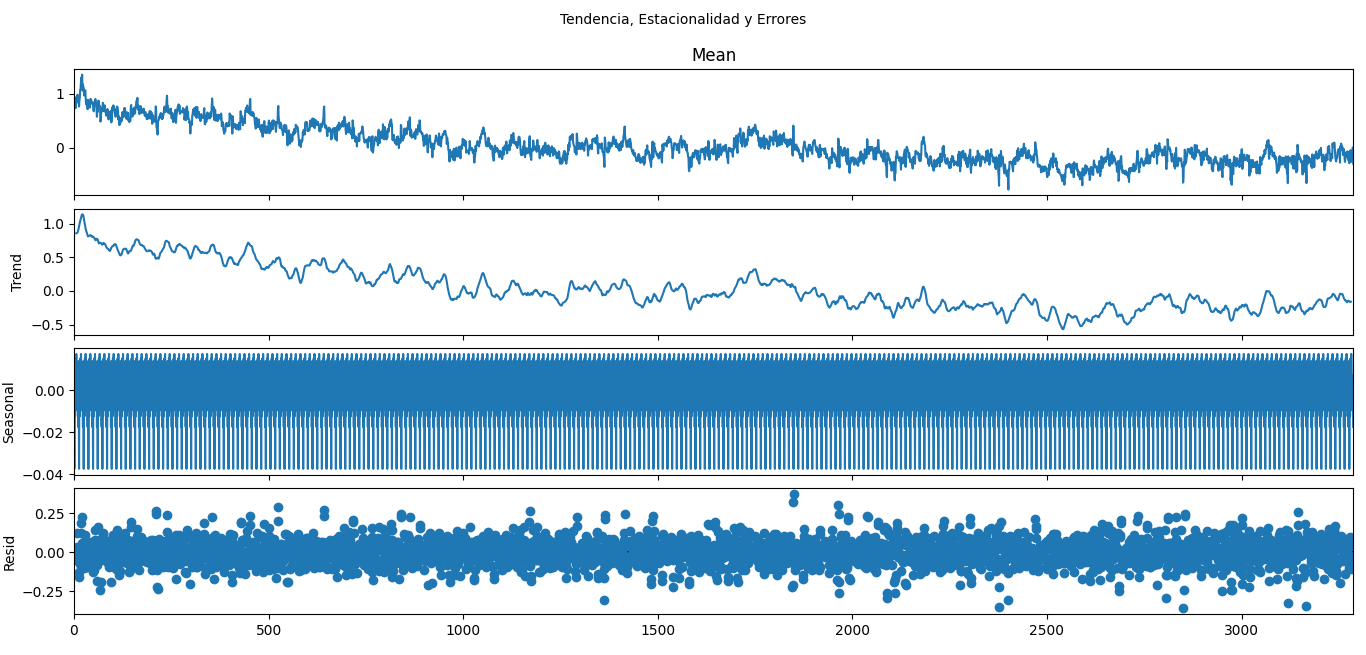
\includegraphics[width = 18 cm ]{Figures/DescomposicionToda.png}
    \caption{Descomposición de la serie de tiempo para las anomalías en las temperaturas mensuales.}
    \label{Fig:8.1}
  \end{figure}

  Vemos que la estacionalidad no esta tan clara en está descomposición para todos los datos. Podemos hacer el análisis solo para los datos que pertenecen a la fuente GCAG.
  
  \begin{figure}[H]
    \centering
    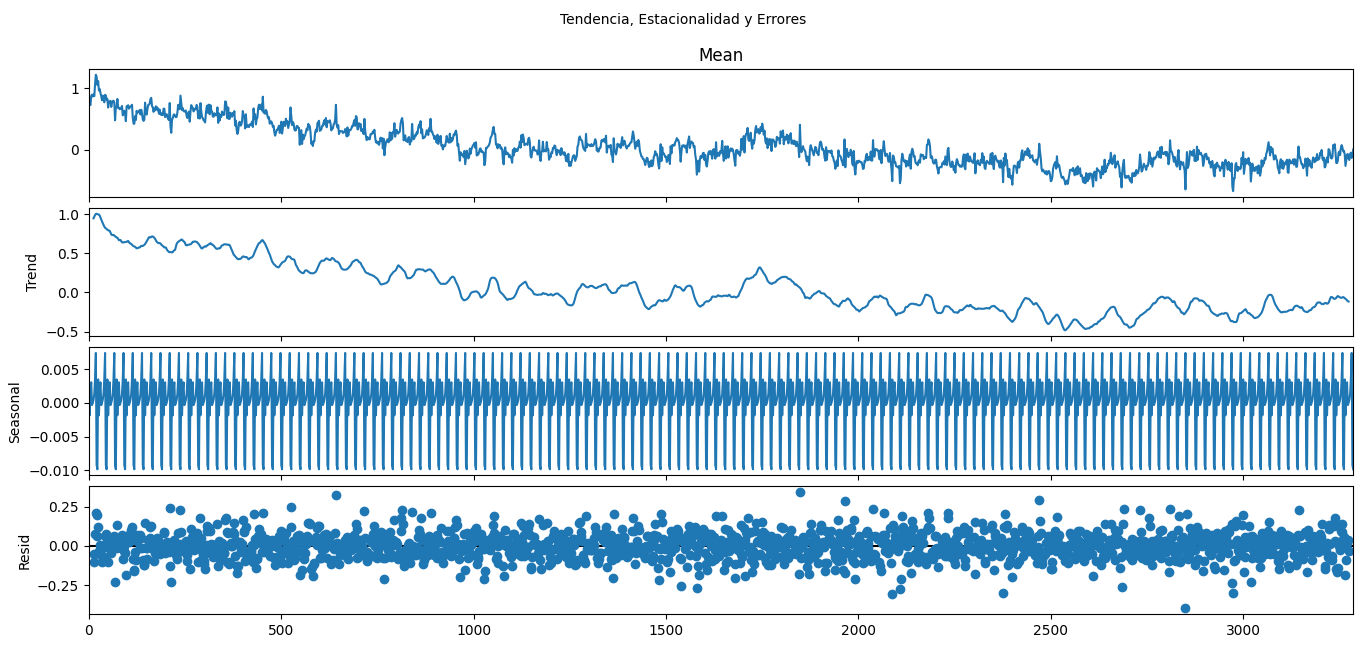
\includegraphics[width = 18 cm ]{Figures/Descomposicion.png}
    \caption{Descomposición de la serie de tiempo para las anomalías en las temperaturas mensuales obtenidos de GCAG.}
    \label{Fig:8.2}
  \end{figure}

  La estacionalidad está mas clara pues vemos que hay saltos equidistantes cada 12 meses.

  Por último para la fuente GISTEMP tenemos la descomposición

  \begin{figure}[H]
    \centering
    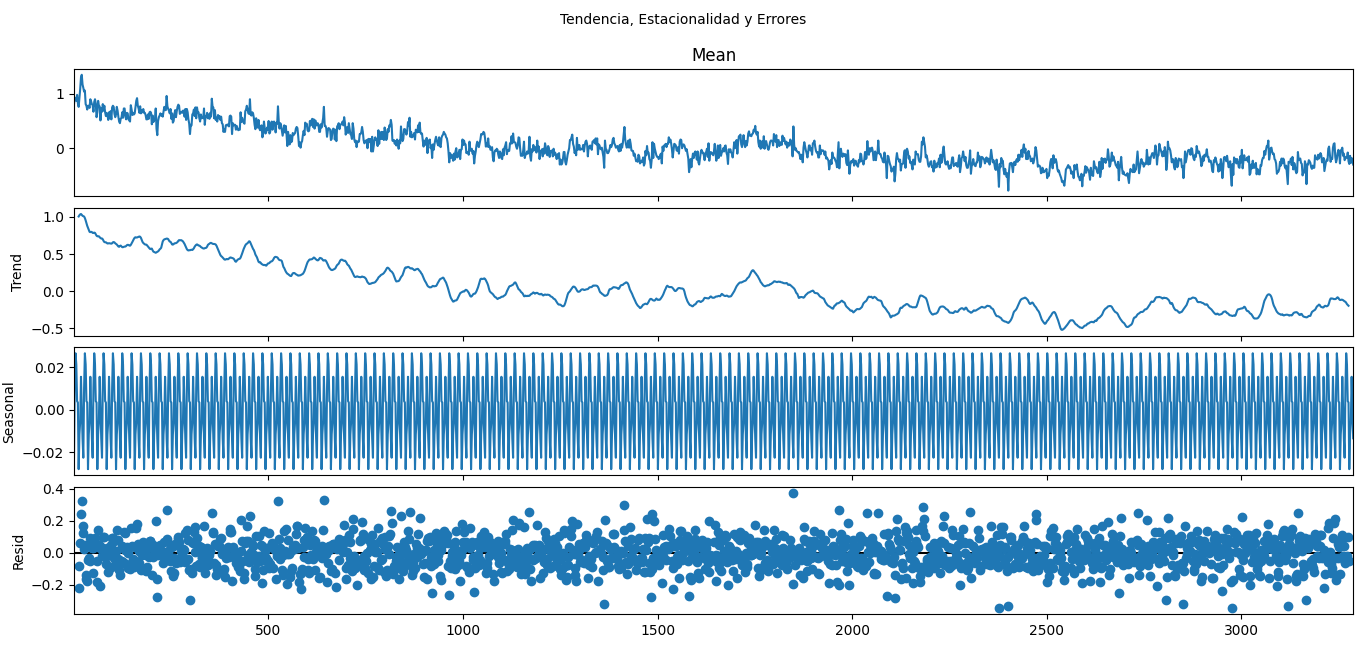
\includegraphics[width = 18 cm ]{Figures/Descomposicion2.png}
    \caption{Descomposición de la serie de tiempo para las anomalías en las temperaturas mensuales obtenidos de GISTEMP.}
    \label{Fig:8.3}
  \end{figure}

  Vemos que la estimación	de la tendencia en cualquier filtración de los datos va a la baja. Es decir, hay menos anomalías climaticas conforme pasan el año. Los errores no aparentan ningun patron por lo que podemos pensar que efectivamente son aleatorios. 

  Por otro lado, vamos a mostrar los correlogramas para la base de datos completa y para cada una de sus fuentes. 

  

  \begin{figure}[H]
    \centering
    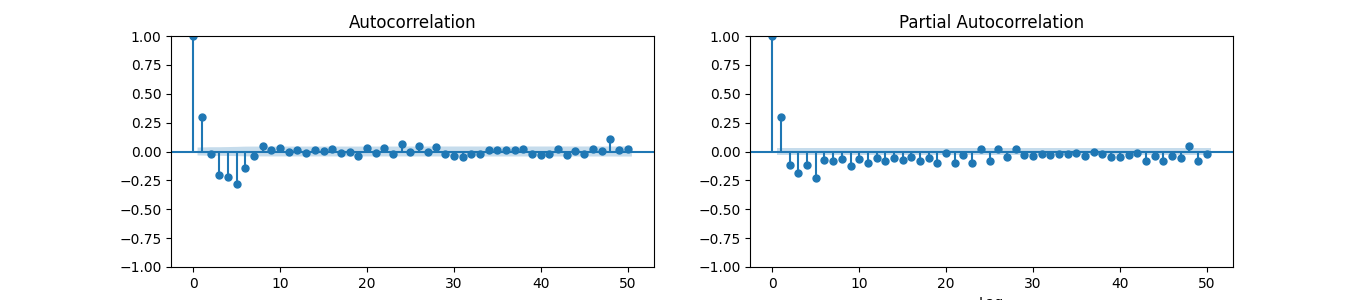
\includegraphics[width = 18 cm ]{Figures/correlo1.png}
    \caption{Correlograma para los errores del modelo aditivo de la serie de tiempo para las anomalías en las temperaturas mensuales obtenidos por ambas fuentes.}
    \label{Fig:8.4}
  \end{figure}


  \begin{figure}[H]
    \centering
    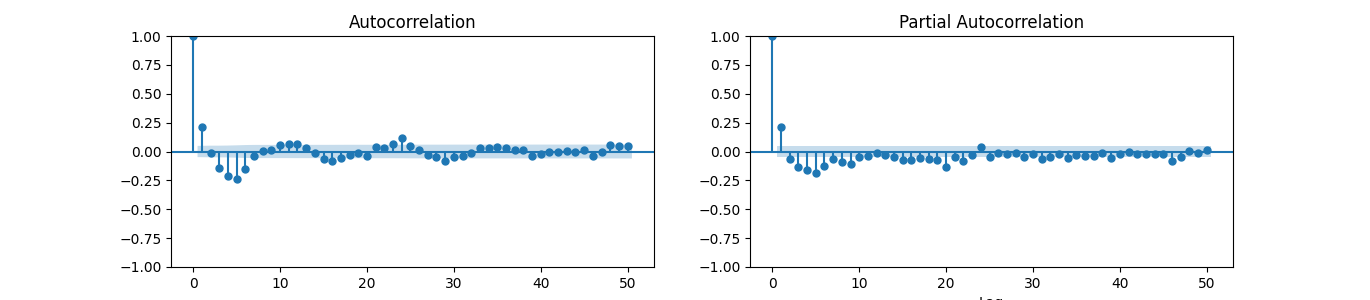
\includegraphics[width = 18 cm ]{Figures/correlo2.png}
    \caption{Correlograma para los errores del modelo aditivo de la serie de tiempo para las anomalías en las temperaturas mensuales obtenidos por fuente GCAG.}
    \label{Fig:8.5}
  \end{figure}


  \begin{figure}[H]
    \centering
    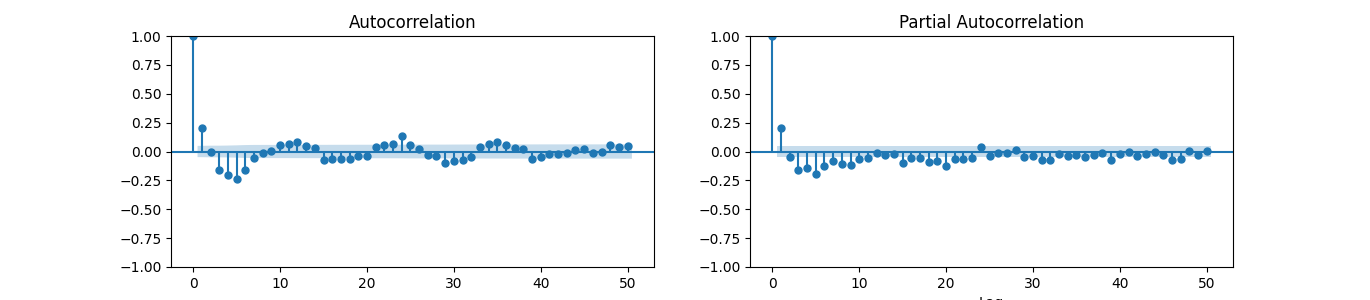
\includegraphics[width = 18 cm ]{Figures/correlo3.png}
    \caption{Correlograma para los errores del modelo aditivo de la serie de tiempo para las anomalías en las temperaturas mensuales obtenidos por la fuente GISTEMP.}
    \label{Fig:8.6}
  \end{figure}
  Vemos que estos correlogramas y correlogramas parciales decaen a cero por lo que pudiese pensarse que provienen de series de tiempo estacionarias, sin embargo se require una prueba formal para aceptar o descartar dicho caso.

\end{solution}


\begin{problem}{9}
    Demuestra todas las identidades de órdenes de probabilidad que no tienen demostración en las notas.
\end{problem}



\end{document}